% !TEX program = pdflatex
\documentclass[3p,11pt]{elsarticle}
\usepackage{amsmath,amssymb}
\usepackage{array}
\usepackage{booktabs}
\usepackage[tableposition=top]{caption}
\usepackage{graphicx}
\usepackage{url}
\urlstyle{same}
\usepackage[hidelinks]{hyperref}
\emergencystretch=3em
% first-page footer: the page number alone
\makeatletter
\def\ps@pprintTitle{\let\@oddhead\@empty\let\@evenhead\@empty
  \def\@oddfoot{\hfil\thepage\hfil}\let\@evenfoot\@oddfoot}
\makeatother

% ---- notation ---------------------------------------------------------------
\newcommand{\kms}{km\,s$^{-1}$}
\newcommand{\ms}{m\,s$^{-1}$}
\newcommand{\Msun}{M$_\odot$}
\newcommand{\Rsun}{R$_\odot$}
\newcommand{\Lsun}{L$_\odot$}
\newcommand{\Mearth}{M$_\oplus$}
\newcommand{\Mjup}{M$_\mathrm{J}$}

\begin{document}

\begin{frontmatter}

\title{A candidate planet of half a Jupiter mass on a 1\,000-day orbit around the K dwarf HD\,76849,
from 21 nights of public HARPS velocities}

\author{Charles C. Norton}

\begin{abstract}
HD\,76849 (HIP\,44059) is a quiet K0 dwarf at 49.1\,pc. Its public HARPS velocities, from 21 nights
between 2007 and 2016, carry a signal near 1\,010\,d with a semi-amplitude of 8.9\,\ms, which a planet
of at least 0.39\,\Mjup\ at 1.9\,au would make. The signal stands in SERVAL's velocities, the HARPS
pipeline's and line-by-line velocities measured here, at false-alarm levels of $10^{-4}$,
$2\times10^{-5}$ and $2\times10^{-4}$. A circular orbit near 1\,010\,d fits better than one at any other
period by $\Delta\chi^2 \geq 18$, and the one-year aliases fit worse by 23 and 25 in log-likelihood.
The pipeline's line width takes two values that change between consecutive nights and follows the
orbit through them; with an offset for each, the signal stays at 1\,013\,d and 8.7\,\ms. The
Hipparcos-Gaia proper-motion anomaly, at $0.7\sigma$, joined to the velocities, holds the companion's
true mass at 0.4 to 0.7\,\Mjup. The nights fall in nine runs, eccentric orbits at 700 and 1\,200\,d
fit nearly as well as the best, and the second half of the nights cannot measure the amplitude, so the
planet is a candidate; velocities over one or two seasons would fix its period and eccentricity.
\end{abstract}

\begin{keyword}
Techniques: radial velocities \sep Planets and satellites: detection \sep Stars: individual: HD\,76849
\end{keyword}

\end{frontmatter}

\section{Introduction}\label{sec:intro}

HARPS-RVBank~\cite{Trifonov2020} recomputed every public HARPS velocity with
SERVAL~\cite{Zechmeister2018}, corrected the instrument's nightly zero points and attached each
spectrum's activity indicators, so that a star's whole record can be read at once. Most of the stars
it holds were observed by several programmes, a few nights at a time. HD\,76849 is one of them: nine
programmes observed it on 21 nights between 2007 and 2016, and no planet has been reported around it.
Its velocities carry a signal that a planet of about half a Jupiter mass on a 1\,000-day orbit would
make. This note gives the signal, the tests it passes and those it cannot yet pass.

\section{Data and the star}\label{sec:data}

HARPS-RVBank holds 21 velocities of HD\,76849, one a night, from 2007 September 22 to 2016 December 17,
with a median error of 1.06\,\ms; five nights follow HARPS's fibre upgrade of 2015
June~\cite{LoCurto2015}, across which the velocities take an offset of their own. The nights fall in
nine runs: 2007 September (three nights), 2008 April (two), 2011 March (one), 2012 March (three), 2012
May (two), 2013 May and June (four), 2013 September (one), 2015 November (four) and 2016 December
(one). DACE holds the HARPS pipeline's cross-correlation velocities of 22 nights, with the Mount Wilson
S index of each spectrum. Line-by-line velocities were measured here from the ESO Science Archive's
spectra of the 21 nights in the manner of line-by-line velocimetry~\cite{Artigau2022}, each spectrum's
shift in each of 4\,816 lines being Bouchy's derivative estimate~\cite{Bouchy2001}; every spectrum was
wavelength-calibrated with a ThAr exposure taken within 0.6 days before it. No other public velocities
of the star exist.

Table~\ref{tab:star} gives the star. Gaia DR3~\cite{GaiaDR3} places it at $49.14 \pm 0.04$\,pc with a
renormalised unit weight error of 0.86, no non-single-star solution and a radial velocity constant over
20 transits, and its astrophysical parameters~\cite{Creevey2023} give 5\,160\,K, $\log g = 4.46$ and
$[\mathrm{M/H}] = -0.03$, 0.93\,\Rsun\ and 0.55\,\Lsun; Gaia's spectroscopic parameters give 5\,221\,K
and $[\mathrm{M/H}] = +0.09$. Gaia gives no mass, and the velocities are read with
$0.85 \pm 0.05$\,\Msun, that of a K0 to K1 dwarf of this temperature and
luminosity~\cite{Pecaut2013}. The S index of its 22 spectra has a median of 0.167,
$\log R'_\mathrm{HK} = -5.02$ for $B-V = 0.843$~\cite{Noyes1984}, the activity of an inactive star,
for which the activity-rotation relation~\cite{Mamajek2008}, at the edge of its range, gives a rotation
period near 45\,d.

\begin{table}[!htbp]
\centering
\caption{HD\,76849.}\label{tab:star}
\begin{tabular}{l r l}
\toprule
Parameter & Value & Source \\
\midrule
Gaia DR3 & 5733849170579848448 & \cite{GaiaDR3} \\
$G$, $G_\mathrm{BP} - G_\mathrm{RP}$ (mag) & 8.83, 1.00 & \cite{GaiaDR3} \\
$V$, $B-V$ (mag) & 9.06, 0.843 & \cite{Perryman1997} \\
Parallax (mas) & $20.351 \pm 0.016$ & \cite{GaiaDR3} \\
RUWE & 0.86 & \cite{GaiaDR3} \\
$T_\mathrm{eff}$ (K) & 5\,160 & \cite{Creevey2023} \\
$\log g$ & 4.46 & \cite{Creevey2023} \\
$[\mathrm{M/H}]$ & $-0.03$ & \cite{Creevey2023} \\
Radius (\Rsun) & $0.926 \pm 0.019$ & \cite{Creevey2023} \\
Luminosity (\Lsun) & $0.548 \pm 0.005$ & \cite{Creevey2023} \\
Mass (\Msun) & $0.85 \pm 0.05$ & \cite{Pecaut2013} \\
S index & 0.167 & HARPS, DACE \\
$\log R'_\mathrm{HK}$ & $-5.02$ & this work \\
\bottomrule
\end{tabular}
\end{table}

\section{The signal}\label{sec:signal}

A generalised Lomb-Scargle periodogram~\cite{Zechmeister2009} of SERVAL's nightly velocities from 1.2 to
3\,000\,d, the offset across the fibre upgrade fitted, peaks at 1\,021.5\,d at a false-alarm
level~\cite{Baluev2008} of $2\times10^{-5}$; with that signal's sinusoid fitted, the residuals' highest
peak, at 19.7\,d, stands at 0.36 (Figure~\ref{fig:periodograms}). Table~\ref{tab:models} gives models
fitted by least squares with the two offsets and a jitter. The planet lowers the Bayesian information
criterion~\cite{Schwarz1978} by 49.4 with a circular orbit; a free eccentricity improves the
log-likelihood by 2.9 for two more parameters and raises the BIC by 0.3. A second signal at 19.7\,d
lowers the BIC by a further 19.6 with circular orbits, but its periodogram peak stands at a false-alarm
level of 0.36, which counts the search over periods that the BIC does not, and the model then fits 21
nights with nine parameters and no jitter. It is not claimed.

\begin{figure}[!htbp]
\centering
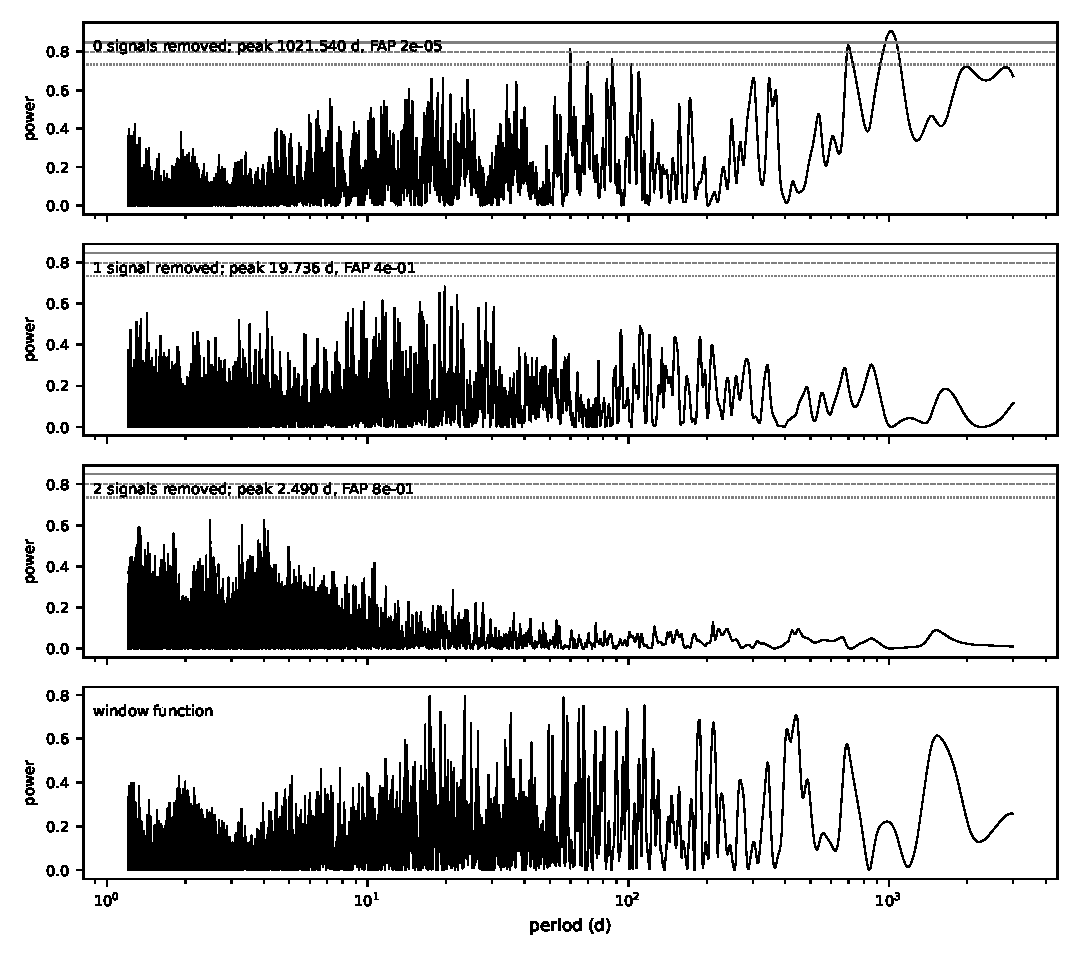
\includegraphics[width=0.92\textwidth]{periodograms.pdf}
\caption{Generalised Lomb-Scargle periodograms of SERVAL's nightly velocities of HD\,76849, each with
the sinusoids of the signals above it fitted jointly, and the observing window's spectral window at the
bottom. The horizontal lines are the false-alarm levels of 0.1, 0.01 and 0.001.}\label{fig:periodograms}
\end{figure}

\begin{table}[!htbp]
\centering
\caption{Models of SERVAL's velocities of HD\,76849: log-likelihood with free and with circular
orbits, the Bayesian information criterion of each, and the free model's jitter and residual scatter.}
\label{tab:models}
\small
\begin{tabular}{l r r r r r r}
\toprule
Periods & $\ln L$ & $\ln L$ (circular) & BIC & BIC (circular) & Jitter (\ms) & Scatter (\ms) \\
\midrule
None & $-69.2$ & $-69.2$ & 147.6 & 147.6 & 6.41 & 6.52 \\
1\,012\,d & $-37.1$ & $-40.0$ & 98.5 & 98.2 & 0.74 & 1.42 \\
1\,015 and 19.8\,d & $-25.1$ & $-25.6$ & 89.7 & 78.5 & 0.00 & 0.82 \\
\bottomrule
\end{tabular}
\end{table}

\subsection{The period}

The nine runs sample the orbit at few phases, so the period was searched directly: at every period from
300 to 6\,000\,d, an orbit's two linear terms were solved with the two offsets and a jitter of
1.55\,\ms, for circular orbits and for eccentricities up to 0.92 at 48 times of periastron. Among
circular orbits the best lies at 1\,011\,d ($\chi^2 = 15.0$ against 248.7 for the offsets alone), and
the best at any other period fits worse by 25.9 or more (702\,d). With eccentric orbits the best lies at
1\,081\,d ($e = 0.6$, $\chi^2 = 9.0$), and orbits at 697\,d ($e = 0.6$, 16.6) and 1\,204\,d ($e = 0.85$,
15.3) fit nearly as well; beyond 1\,700\,d no orbit comes within 15. The one-year aliases of the
periodogram's peak, at 269 and 562\,d, fit worse by 24.9 and 23.2 in log-likelihood. Three hundred sets
of velocities drawn from the circular model with the planet at 1\,015\,d give a ratio of the powers at
1\,015 and 269\,d of $2.2^{+0.4}_{-0.2}$, and 19 per cent of them reach the observed 2.55, while none of
three hundred with the planet at 269\,d does~\cite{Dawson2010}; against 562\,d the observed ratio, 2.37,
lies between the simulations with the planet at 1\,015\,d, all above 9.8, and those with it at 562\,d,
all below 0.39.

\section{The instrument and stellar activity}\label{sec:tests}

The signal stands in each of the three reductions as the highest peak of the periodogram: SERVAL's
velocities at 1\,019\,d and a false-alarm level of $1.2\times10^{-4}$, the pipeline's at 1\,005\,d and
$1.6\times10^{-5}$, and the line-by-line velocities at 1\,005\,d and $1.6\times10^{-4}$. Its first half
of nights, eleven from 2007 to 2012, gives a semi-amplitude of $7.9 \pm 0.7$, $6.6 \pm 0.5$ and
$8.2 \pm 0.6$\,\ms\ in the three; the second half, ten from 2013 to 2016 of which five follow the upgrade
with an offset of their own, covers too little of the orbit to measure it ($22 \pm 25$, $22 \pm 11$ and
$48 \pm 16$\,\ms). The line-by-line test against activity does not apply to this star: 1\,228 of the
4\,816 lines correlate with the S index at $p < 0.01$, and 1\,017 within the 16 spectra before the
upgrade alone, where 48 would by chance, so the index and the lines' shifts share something that is
not the star's activity.

The periodograms of the chromatic index, the differential line width, the H$\alpha$ and Na\,D indices,
the pipeline's bisector and the S index from DACE's spectra and from the line-by-line spectra have no
power near the period (false-alarm levels of 1.0 within 5 per cent of it), and the S index does not
follow the orbit ($r = -0.23$, $p = 0.32$). The pipeline's line width has power there at a false-alarm
level of 0.18 and takes two values, 6.18 to 6.21 and 6.79 to 6.81\,\kms, with two nights at 6.32 and
6.36\,\kms; it changes from one to the other between consecutive nights of one programme, 2013 June 17
and 18, as no star's lines do. Before the upgrade the wider value holds the five nights of 2012, near
the orbit's minimum, and the line width follows the orbit through them ($r = -0.67$, $p = 0.004$).
Fitted with an offset for each value of the line width, the velocities keep the signal: the best
circular orbit lies at 1\,013\,d with a semi-amplitude of 8.7\,\ms, and the best at any other period
fits worse by 17.8 or more.

\section{Orbit and mass}\label{sec:orbit}

Table~\ref{tab:orbit} gives the circular orbit, sampled with emcee~\cite{ForemanMackey2013} and its
differential-evolution moves~\cite{terBraak2006}, 48 walkers over 20\,000 steps, with the two offsets
and a jitter. Sampled with its eccentricity free, the orbit moves to $1\,071^{+25}_{-32}$\,d and
$12.6^{+6.0}_{-2.2}$\,\ms, with an eccentricity of $0.60^{+0.18}_{-0.18}$ and a minimum mass of
$145^{+25}_{-14}$\,\Mearth, but that chain's autocorrelation time, 548 steps, leaves it 18 times as long
after burn-in, and its eccentricity reflects the runs' phases as much as the orbit. Figure~\ref{fig:phased}
shows the velocities phased at the period.

\begin{table}[!htbp]
\centering
\caption{HD\,76849\,b: medians and 68 per cent intervals of the circular orbit sampled from the HARPS
velocities, with the star's mass of 0.85\,\Msun.}
\label{tab:orbit}
\begin{tabular}{l r}
\toprule
Parameter & Value \\
\midrule
Period (d) & $1\,011 \pm 14$ \\
Semi-amplitude $K$ (\ms) & $8.89 \pm 0.62$ \\
Time of conjunction (BJD) & $2455670 \pm 17$ \\
Minimum mass $m \sin i$ (\Mearth) & $125 \pm 9$ \\
Minimum mass $m \sin i$ (\Mjup) & $0.394 \pm 0.029$ \\
Semi-major axis (au) & 1.87 \\
Insolation (Earth's) & 0.16 \\
Equilibrium temperature, no albedo (K) & 175 \\
Transit probability & 0.23 per cent \\
Jitter (\ms) & $1.55^{+0.49}_{-0.40}$ \\
\bottomrule
\end{tabular}
\end{table}

\begin{figure}[!htbp]
\centering
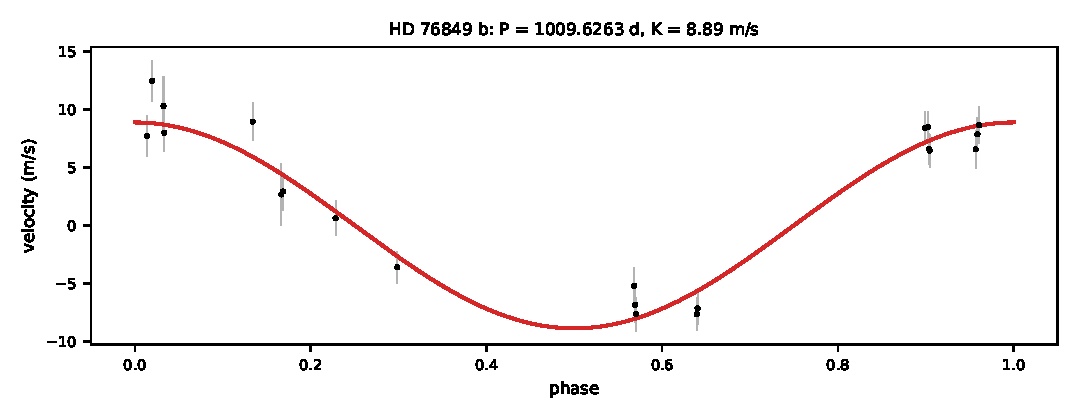
\includegraphics[width=0.8\textwidth]{phased.pdf}
\caption{SERVAL's nightly velocities of HD\,76849, each side of the fibre upgrade's offset removed,
phased at 1\,009.6\,d with the circular orbit fitted by least squares. The error bars include the
jitter.}\label{fig:phased}
\end{figure}

Gaia DR3 holds no acceleration or orbital solution for the star. Its proper-motion anomaly between
Hipparcos and Gaia, computed from Hipparcos's new reduction~\cite{vanLeeuwen2007} and Gaia DR3 as
Kervella et al.\ define it~\cite{Kervella2022}, stands at $0.7\sigma$. One Keplerian orbit, the
companion dark, fitted to the velocities and the anomaly together with the star's mass held to its
prior and the period above 500\,d, gives $1\,071^{+17}_{-18}$\,d, an eccentricity of
$0.55^{+0.10}_{-0.10}$, an inclination of $79^{+34}_{-39}$ degrees and a true mass of
$0.50^{+0.23}_{-0.07}$\,\Mjup\ at $1.93 \pm 0.05$\,au; every sample lies below 13\,\Mjup. An orbit seen
nearly face on, which would make the companion a brown dwarf or a star, would move the star's
photocentre more than the anomaly allows.

TESS~\cite{Ricker2015} observed the star in five sectors from 2019 to 2026, read through
Lightkurve~\cite{Lightkurve2018}. The circular orbit's conjunctions there are uncertain by one to three
months, the sectors cover 13 per cent of the probability of one of them, and the transit probability is
0.23 per cent, so the photometry does not test a transit.

\section{Discussion}\label{sec:discussion}

The 21 nights of HD\,76849 carry a signal near 1\,010\,d in three reductions of the same spectra, which a
planet of at least 0.39\,\Mjup\ at 1.9\,au would make, and the astrometry, joined to the velocities,
holds its true mass at 0.4 to 0.7\,\Mjup. A planet of that mass around a quiet K dwarf at 1.9\,au, where
it would receive a sixth of the Earth's insolation, is of a kind radial-velocity surveys find around a
few per cent of Sun-like stars. Three facts keep it a candidate. The nights fall in nine runs, so that
eccentric orbits at 700 and 1\,200\,d fit nearly as well as the best; the second half of the nights cannot
measure the amplitude; and the line-by-line test against activity does not apply. The line width's two
values follow the orbit and the signal survives them, but they show that the spectra of different runs
were not taken or reduced alike. Velocities on a dozen nights spread over one or two seasons would fix
the period and the eccentricity and confirm the planet.

\section{Conclusion}\label{sec:conclusion}

HD\,76849, a quiet K0 dwarf at 49.1\,pc, carries a signal near 1\,010\,d and 8.9\,\ms\ in 21 nights of
public HARPS velocities, a candidate planet of 0.4 to 0.7\,\Mjup\ at 1.9\,au when the velocities are
joined to the Hipparcos-Gaia astrometry. The period is preferred to every other circular orbit and to
both one-year aliases, and the signal survives an offset for each of the line width's two values; the
sampling leaves eccentric orbits at other periods nearly as good, and new velocities would decide.

\section*{Acknowledgements}

Based on data obtained from the ESO Science Archive Facility, on HARPS-RVBank, and on DACE, the Data \&
Analysis Center for Exoplanets, a facility of the University of Geneva and a platform of the Swiss
National Centre of Competence in Research PlanetS. This work has made use of data from the European Space
Agency missions Gaia, processed by the Gaia Data Processing and Analysis Consortium, funded by national
institutions, in particular the institutions participating in the Gaia Multilateral Agreement, and
Hipparcos; and of the TESS mission, funded by NASA's Science Mission Directorate. The velocities, tests
and orbits were computed with orbitlight's planets mode.

\begin{thebibliography}{99}\small\raggedright
\setlength{\itemsep}{1pt}

\bibitem{Trifonov2020}
T.~Trifonov et al., Public HARPS radial velocity database corrected for systematic errors,
\emph{Astron. Astrophys.} \textbf{636}, A74 (2020).

\bibitem{Zechmeister2018}
M.~Zechmeister et al., Spectrum radial velocity analyser (SERVAL). High-precision radial velocities and
two alternative spectral indicators, \emph{Astron. Astrophys.} \textbf{609}, A12 (2018).

\bibitem{LoCurto2015}
G.~Lo Curto et al., HARPS gets new fibres after 12 years of operations, \emph{The Messenger}
\textbf{162}, 9 (2015).

\bibitem{Artigau2022}
\'E.~Artigau et al., Line-by-line velocity measurements: an outlier-resistant method for precision
velocimetry, \emph{Astron. J.} \textbf{164}, 84 (2022).

\bibitem{Bouchy2001}
F.~Bouchy, F.~Pepe and D.~Queloz, Fundamental photon noise limit to radial velocity measurements,
\emph{Astron. Astrophys.} \textbf{374}, 733 (2001).

\bibitem{GaiaDR3}
Gaia Collaboration, A.~Vallenari et al., Gaia Data Release 3. Summary of the content and survey
properties, \emph{Astron. Astrophys.} \textbf{674}, A1 (2023).

\bibitem{Creevey2023}
O.~L. Creevey et al., Gaia Data Release 3. Astrophysical parameters inference system (Apsis). I. Methods
and content overview, \emph{Astron. Astrophys.} \textbf{674}, A26 (2023).

\bibitem{Pecaut2013}
M.~J. Pecaut and E.~E. Mamajek, Intrinsic colors, temperatures, and bolometric corrections of
pre-main-sequence stars, \emph{Astrophys. J. Suppl. Ser.} \textbf{208}, 9 (2013).

\bibitem{Noyes1984}
R.~W. Noyes et al., Rotation, convection, and magnetic activity in lower main-sequence stars,
\emph{Astrophys. J.} \textbf{279}, 763 (1984).

\bibitem{Mamajek2008}
E.~E. Mamajek and L.~A. Hillenbrand, Improved age estimation for solar-type dwarfs using
activity-rotation diagnostics, \emph{Astrophys. J.} \textbf{687}, 1264 (2008).

\bibitem{Perryman1997}
M.~A.~C. Perryman et al., The Hipparcos catalogue, \emph{Astron. Astrophys.} \textbf{323}, L49 (1997).

\bibitem{Zechmeister2009}
M.~Zechmeister and M.~K\"urster, The generalised Lomb-Scargle periodogram. A new formalism for the
floating-mean and Keplerian periodograms, \emph{Astron. Astrophys.} \textbf{496}, 577 (2009).

\bibitem{Baluev2008}
R.~V. Baluev, Assessing the statistical significance of periodogram peaks, \emph{Mon. Not. R. Astron.
Soc.} \textbf{385}, 1279 (2008).

\bibitem{Schwarz1978}
G.~Schwarz, Estimating the dimension of a model, \emph{Ann. Statist.} \textbf{6}, 461 (1978).

\bibitem{Dawson2010}
R.~I. Dawson and D.~C. Fabrycky, Radial velocity planets de-aliased: a new, short period for super-Earth
55 Cnc e, \emph{Astrophys. J.} \textbf{722}, 937 (2010).

\bibitem{ForemanMackey2013}
D.~Foreman-Mackey, D.~W. Hogg, D.~Lang and J.~Goodman, emcee: the MCMC hammer, \emph{Publ. Astron. Soc.
Pac.} \textbf{125}, 306 (2013).

\bibitem{terBraak2006}
C.~J.~F. ter Braak, A Markov chain Monte Carlo version of the genetic algorithm Differential Evolution:
easy Bayesian computing for real parameter spaces, \emph{Stat. Comput.} \textbf{16}, 239 (2006).

\bibitem{vanLeeuwen2007}
F.~van Leeuwen, Validation of the new Hipparcos reduction, \emph{Astron. Astrophys.} \textbf{474}, 653
(2007).

\bibitem{Kervella2022}
P.~Kervella, F.~Arenou and F.~Th\'evenin, Stellar and substellar companions from Gaia EDR3.
Proper-motion anomaly and resolved common proper-motion pairs, \emph{Astron. Astrophys.} \textbf{657},
A7 (2022).

\bibitem{Ricker2015}
G.~R. Ricker et al., Transiting Exoplanet Survey Satellite, \emph{J. Astron. Telesc. Instrum. Syst.}
\textbf{1}, 014003 (2015).

\bibitem{Lightkurve2018}
Lightkurve Collaboration, Lightkurve: Kepler and TESS time series analysis in Python, Astrophysics
Source Code Library, ascl:1812.013 (2018).

\end{thebibliography}

\end{document}
